


This book uses three ideas: (1) critical complexity to assess the limits of models; (2) a modelling approach that combines machine-learning and mechanistic models;  and (3) relational ethics to look at how modellers engage (and sometimes fails to engage) with the world. In this chapter, we give a broad outline of these three ideas, on which we will build upon as we go. 

\section{Critical complexity}

Biological and social systems are complex. The human brain and our other organs; the web of soical interactions over the Internet; the structure of a large buisness or the activities at a University; the ecosystems we live in and are part of; the growth of an embryo; the inner workings of an ant colony or the movement of a fish school. Each one of these systems consist of interacting units that produce patterns far more complex than the units themselves. They are shaped by history. They are messy and difficult to characterise. It is difficult to know where they start and end. 

The scientific challenge is to use the fact that a system is complex to help us better understand it. Sometimes, when we say that a system is complicated when we mean that our insight in to that system is limited. A complex system is difficult to understand. What then can be gained by thinking in terms of complexity science?

The answer to that question, which we underlies the approach taken in this course, comes in the form of {\bf critical complexity}. The term critical complexity arises out of the work of philosophers Paul Cilliers\cite{cilliers2002complexity,cilliers2016critical,cilliers2005complexity}, Alicia Juarrero\cite{juarrero1999dynamicsbook,juarrero2000dynamics} and Rika Preiser\cite{preiser2012problem,preiser2013deconstruction}. These philosophers emphasise the need to embrace the ambiguous, messy, fluid, non-determinable, contextual, and historical nature of complex systems. They describe complex phenomena as unfinalizible and inexhaustible. Complex systems are open-ended, which means there is no way of making an uncontested description of that system. There are always new and different ways of looking at the system.

A way of visualising this description of a complex system is provided by Di Paolo et al. (2018) and reproduced in figure \ref{fig:Complexity}. In the figure, the agents (circles) in a complex system interact (straight arrows) with each other, their environment (wavy lines), which is partially open and ever-changing, and these interactions are continually adjusted (curved arrows) by the agents themselves. 


\begin{figure}[t]
\centering
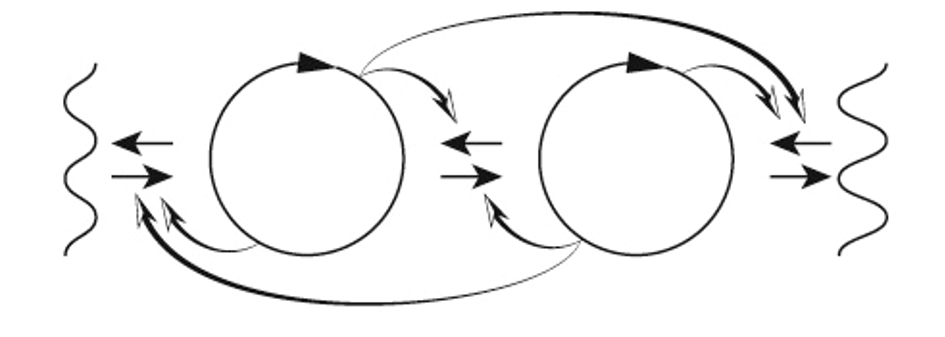
\includegraphics[width=10cm]{Figures/Complexity/Complexity.png}
\centering
\caption{An illustration of a complex system. Adapted from Di Paolo et al. (2018) \cite{di2018linguistic}.  \label{fig:Complexity}}
\end{figure}

If we were to now try to model such a system, or describe some aspect of it, we are forced to make choices about what is inside our model and what is outside. The figure below illustrates such choices, with the blue squares representing ways in which we have closed the system in order to make a model.



\begin{figure}[p]
\centering
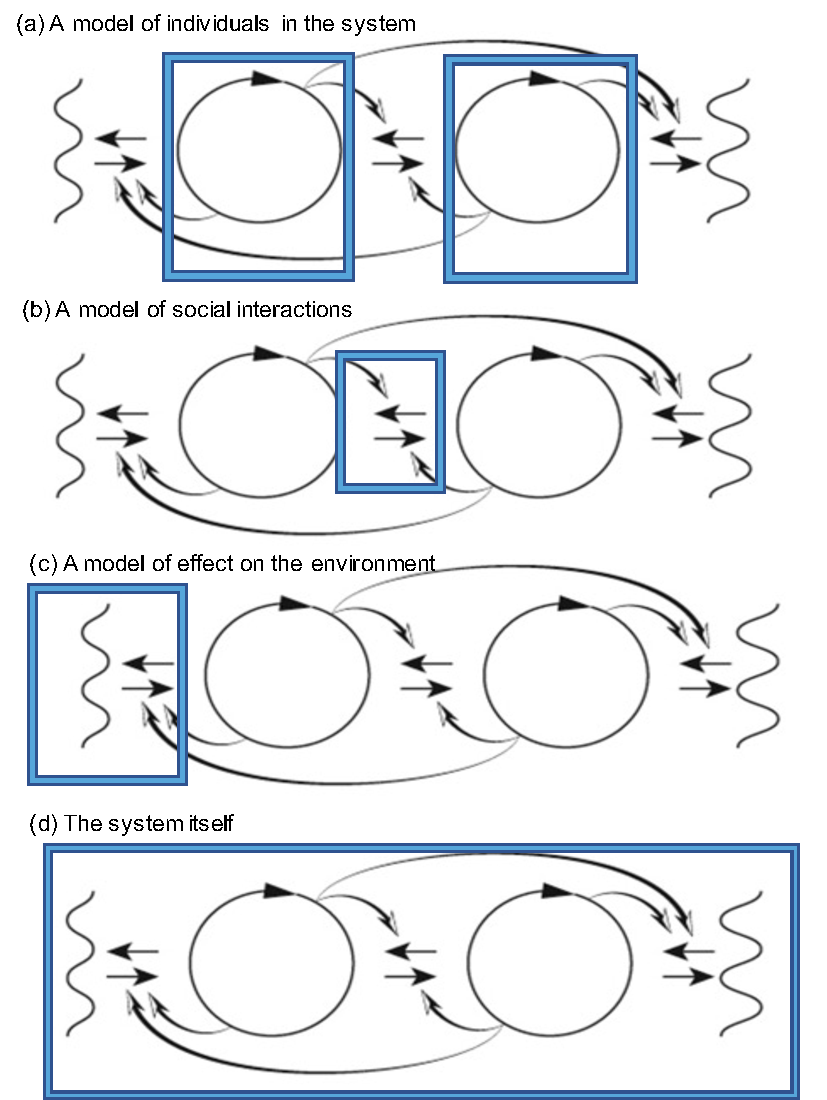
\includegraphics[width=12cm]{Figures/Complexity/ModelsOfComplexity.pdf}
\centering
\caption{Four different ways of modelling a complex system. In terms of (a) individuals (b) social interactions (c) effect of environment or (d) as the entire system. \label{fig:ModelsOfComplexity}} 

\end{figure}


In figure \ref{fig:ModelsOfComplexity} (a) we focus on the individual agents and how they behave, so we create a model which describes their properties and makes simplifying assumptions about how they interact with each other and the world. Here, the agents are inside the model, while their interactions and the environment is outside. In figure \ref{fig:ModelsOfComplexity}(b) we focus instead on the interactions between the agents and in (c) we look at the effect the agents have on their environment. Again, in both these cases, we make simplifying assumptions about things on the outside in order to create a model of the inner workings of one part of the system. 

It is in this way that complex phenomena are unfinalizible and inexhaustible. There are infinitely many ways of building up models of a system, each which leaves something outside. A model is like a snapshot of a landscape and no single snapshot tells the whole story. For modelling the human body, for example, ``a portrait of a person, a store mannequin, and a pig can all be models” \cite{blanchard2011differential}. None is a perfect representation, but each can be the best model for a human, depending on whether one wants to remember an old friend, to buy clothes, or to study anatomy. 

The critical complexity view says that, because complex systems cannot not be completely measured and carry their history with them, there is always a new and different way of looking at them. A few years (or even days) after a portrait is drawn, a person is no longer the same as they were then. We can even talk about their relationship to that portrait, how it shapes their view of the world as they age. The act of modelling, of discussing and analysing changes the world itself. We can never fully capture reality in a single snapshot.

The exception to this rule is illustrated in figure \ref{fig:ModelsOfComplexity}(d), in which we make a model of the entire system. Cilliers argues that such a model {\it is} the system itself. To create such a model, we would need to describe every historical, sociological, biological and physical detail of that system. We would even have to include ourselves studying the system in the model. It is impossible in practice to build such a model and it would be equally impossible to make use of the model or understand what it is telling us.

The use of the word 'critical' in 'critical complexity' thus refers to an activity of criticising a failure to recognise limitations in our models and of thinking carefully about the way we approach modelling. It is this approach we take throughout this book. We see the world as complex in the sense that it is  ambiguous, unfinalizible and inexhaustible. And we are critical of ways in which modellers can fail to recognise complexity and the consequences such failure has on how models are used in society. 

\section{Machine learning and modelling}

\label{sec:mathmodels}

Machine learning is an approach to building models of both simple and complex systems. Let's illustrate how some of these methods work. Not in mathematical detail, but conceptually.


\begin{figure}[t]
\centering
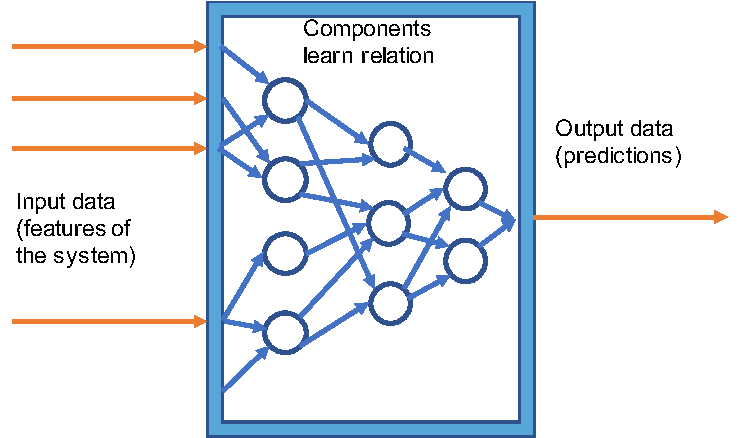
\includegraphics[width=10cm]{Figures/Complexity/SupervisedLearning.pdf}
\centering
\caption{An illustration of the supervised learning problem.   \label{fig:SupervisedLearning}}
\end{figure}


The most well-known method is {\it supervised machine learning}. The idea here is to learn 


In the interactive worksheet (LINK), we give an example of a supervised learning method (logistic regression) in football. MORE  


\begin{figure}[t]
\centering
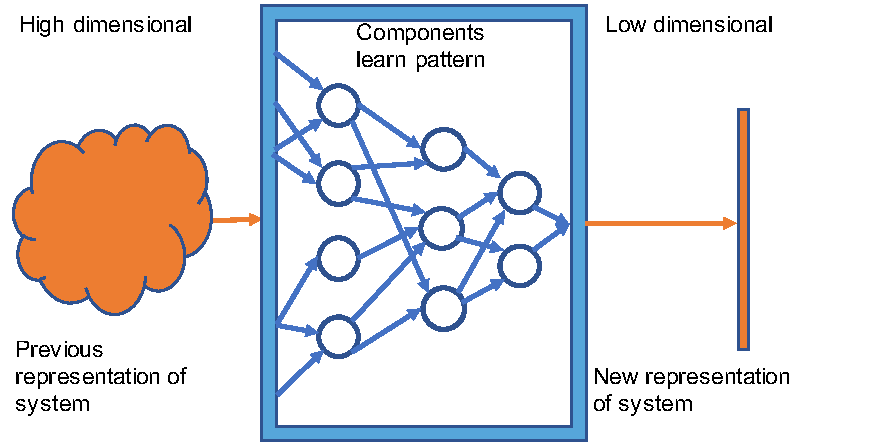
\includegraphics[width=10cm]{Figures/Complexity/UnsupervisedLearning.pdf}
\centering
\caption{An illustration of the supervised learning problem.   \label{fig:UnsupervisedLearning}}
\end{figure}

In {\it unsupervised machine learning} ...

In the interactive worksheet (LINK), we provide an example of categorising a group of people based on their interests using principal component analysis (PCA). MORE HERE.

There are a variety of methods for unsupervised learning. 


In {\it mechanistic modelling}.

\begin{figure}[t]
\centering
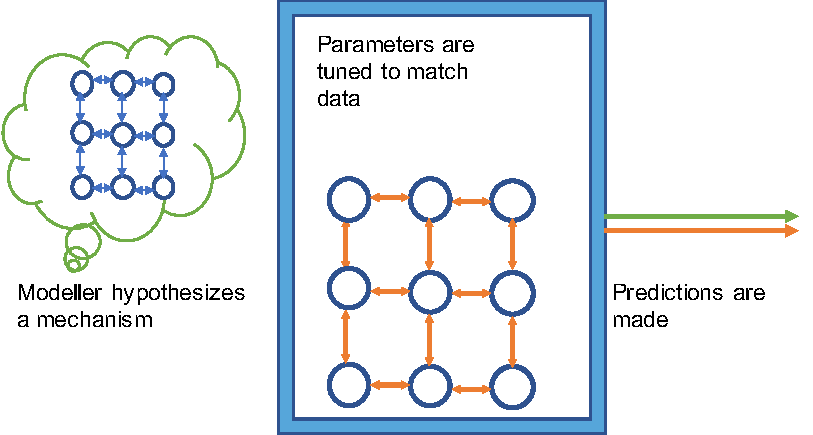
\includegraphics[width=10cm]{Figures/Complexity/Mechanism.pdf}
\centering
\caption{An illustration of a mechanistic model.   \label{fig:Mechanism}}
\end{figure}


In the interactive worksheet (LINK), we provide an example of a mechanistic model of disease spread using an SIR model.

Return to football example. This time with the angle.


OTHER EXAMPLES


\section{An open approach}

In this book, we take an approach to mathematical modelling and machine learning that builds upon figure \ref{fig:ModelsOfComplexity}. We will start from the assumption that there is no unique way of viewing a complex system, but many different views, each of which gives a different insight. Moreover, we assume that applying a mathematical model is akin to using a camera to take a picture of a system. Figures \ref{fig:SupervisedLearning}, \ref{fig:UnsupervisedLearning} and \ref{fig:Mechanism} give an outline of how some these different cameras are built, while the examples in the previous section show in more detail how they work.

In the next chapter we focus on identifying ways in which models close systems. Some systems --- board games, short scale weather prediction, specific datasets and to some extent, biological processes, such as protein folding --- are amenable to closure. We can define where a closed system starts and ends and draw a box around it, which defines its inputs, its outputs and its function. It is conceptually straightforward (although often technically challenging) to build models of these closed systems, which help us understand their properties and predict how they will behave. Then, in chapter \ref{chap:Open}, we look at other systems --- football matches, the Hollywood film industry, the movement of animal groups, outcomes of peoples lives, changes in society--- that are open. It is much harder to build models of these systems, both conceptually and in practice. In many cases it is impossible.

We will argue that the best way to approach complex, open systems is by constructing a wide variety of views. Adopting this approach leads us to a central theme in this book: that when we make choices about which camera to use and which view to take, we cannot escape the fact we are including ourselves in the modelling process. There is no single, objective view to take of these systems. Our values and our ethical choices become part of the modelling process.

Thus, when we look at the technical possibilities and limitations of modelling, we also have to consider ethics and values. We will explain this approach, known as relational ethics, in more detail in chapter \ref{chap:Relational}. But in order to allow the reader to see where we are going with the examples of open and closed systems in the next two chapters, we now give a broad outline of the central idea of relational ethics.

\section{Relational Ethics}

\label{relational}

Relationalism is the idea that morality is an interactive property established between two or more individuals \cite{metz2016relational}. More concretely, the relational approach can be framed in terms of the Ubuntu world view that ``I am
because we are, and since we are, therefore I am'' \cite{mbiti1969african}. Ubuntu is an African philosophy, best known in the West through Archbishop Desmond Tutu’s speech {\it No Future Without Forgiveness}, in which he said, 

\begin{quote}

I am fully me only if you are all you can be. Anger, resentment, nursing grudges corrode, subvert the summum bonum, the great good of the African worldview of communal harmony and they eat away at the very vitals. To forgive is not being altruistic; it is the best form of self-interest. You know what happens to your blood pressure when you are caught in a traffic jam, ``How come they let all those morons drive a car?'' To forgive is good for your physical health as it is for your spiritual health.

\end{quote}

Tutu's description of Ubuntu has parallels to the view of a complex system we saw in figure \ref{fig:Complexity}. It asks us to think of ourselves, when stuck in a traffic jam, as both consisting of a biochemical system (measured by our blood pressure) and as part of an overall social system, our interactions with the other drivers. When analysing the morality of a situation (even one as terrible as Apartheid), Tutu's allegory says we should not just focus on one level, but instead take a view of the various relationships within the system. Just as we should remember that our models capture only one part a larger system or omit detail at a lower level (as in figure \ref{fig:ModelsOfComplexity}), it is a mistake to analyse traffic jams only in terms of ``moron'' drivers. 

Relational frameworks emphasize the importance of dependencies. For example, Kyselo \cite{kyselo2014body} contends that the self is social through and through. We become ourselves and sustain ourselves together with others. Similarly, Bakhtin \cite{bakhtin1984problems} says that only through encounters with others, can we appreciate our own perspectives and form a coherent image of ourselves as a whole entity. By \textit{`looking through the screen of the other’s soul,'} he wrote, \textit{`I vivify my exterior'}. Selfhood and knowledge are evolving and dynamic; the self is never finished – it is an open book \cite{birhane2017descartes}. 

Consider these relational views of our place in society in the context of, for example, predictive policing. The view taken when creating an algorithm to predict crime locations in a city is similar to that of Batman, patrolling a society from the outside and viewing crimes from above in terms of hot spots on a map. Instead of being part of the community, the predictive policing view is disconnected from it. Batman is alienated from those he should serve. As we shall see in chapter \ref{chap:Prediction}, this alienation leads to poor predictions and stereotyping in the use of predictive policing. In order to create successful models of society, we need to consider our own (and our models) place in it. 

In the context of such examples, a particularly important relational approach is Afro-feminism thought. This approach maintains that the most reliable form of knowledge, especially in relation to social and historical injustices, is grounded in lived experience. Patricia Hill Collins \cite{collins2002black}, emphasizes that people do not see the world in abstract forms from a distance, but instead knowledge and understanding emerge from concrete lived experiences. The Afro-feminist approach contends that concrete experiences are primary and abstract reasoning (including modelling) is secondary. Knowing and being are active processes, that are necessarily political and ethical. 

According to the approach outlined by Collins, mathematical models (such as those we discussed in section \ref{sec:mathmodels}) do not take precedence over the actual experience of a person. Modelling cannot be carried out in isolation from others, but should be developed in dialogue with the community it impacts. This is especially important when the type of knowledge in question concerns oppression, structural discrimination, and racism. The Afro-feminist approach maintains that concepts such as ethics and justice need to be grounded in concrete events informed by lived experience of the most marginalized, individuals and communities. We will return to Afro-feminism in more detail in section \ref{sec:Afro-feminism}.

In a similar vein to Afro-feminist thought, the enactive cognitive science theory of participatory sense-making \cite{de2007participatory} advocates for an active and engaged knowing rooted in our relating. A proponent of this position, Hanne De Jaegher \cite{de2019loving}, contends that our most sophisticated human knowing lies in how we engage with each other. In \textit{`Loving and knowing: Reflections for an engaged epistemology'}, De Jaegher \cite{de2019loving} emphasizes that discrete, rational knowing comes at the detriment of \textit{Knowing-in-connection}. Far from a distant and ``objective'' discretising logic, knowing is an activity that happens in the relationship between the knower and the known. Proposing an understanding of human knowing in analogy with loving, De Jaegher argues that in knowing, like loving, what happens is not neutral, general, or universal. Knowers, like lovers, are not abstract subjects but are particular and concrete. ``\textit{Who loves matters}.'' And both loving and knowing take place in the relation between them \cite{de2019loving}. 

Human knowing is based not on purely rational logic, as the rational worldview assumes, but on living and connected know-hows. ``Our most sophisticated knowing'', according to De Jaegher, ``\textit{is full of uncertainty, inconsistencies, and ambiguities}.'' One of the consequences of prioritizing reason is that knowledge of the world and of other people becomes something that is rooted in the individual person’s rational reasoning – in direct contrast to engaged, active, involved, and implicated knowing. Humans are inherently historical, social, cultural, gendered, politicized, and contextualized organisms. Accordingly, their knowing and understanding of the world around them necessarily takes place through their respective lenses.

People are not solo cognizers that manipulate symbols in their heads and perceive their environment in a passive way, as the rationalist view would suggest, but they actively engage with the world around them in a meaningful and unpredictable way. Living bodies, according to Di Paolo, Cuffari, and De Jaegher \cite{di2018linguistic}, are processes, practices, and networks of relations which have ``more in common with hurricanes than with statues''. They are unfinished and always becoming, marked by\textit{``innumerable relational possibilities, potentialities and virtualities''} and not calculable entities whose behaviour can neatly be categorized and predicted in a precise way. Bodies: ``...grow, develop, and die in ongoing attunement to their circumstances... Human bodies are path-dependent, plastic, nonergodic, in short, historical. There is no true averaging of them.'' \citep[p.97]{di2018linguistic}. 

TEXT ABOVE (FROM ABEBA THESIS) SHOULD BE SHORTENED.

Relational perspectives thus view existence in terms of a complex web of social relations. Thus, as in critical complexity, they highlight the impossibility of any unambiguous separation of the real-world, the models we build of a system, and our human values. Afro-feminsism, in particular, emphasises an inherent connection between how one thinks (builds models) and what one does (how models are used and impact society). It is impossible to build a model of reality without taking a specific view and thus adopting an ethical standpoint. Batman beware.
